\documentclass[preprint, 3p,
authoryear]{elsarticle} %review=doublespace preprint=single 5p=2 column
%%% Begin My package additions %%%%%%%%%%%%%%%%%%%

\usepackage[hyphens]{url}

  \journal{Transport Geography?} % Sets Journal name

\usepackage{graphicx}
%%%%%%%%%%%%%%%% end my additions to header

\usepackage[T1]{fontenc}
\usepackage{lmodern}
\usepackage{amssymb,amsmath}
% TODO: Currently lineno needs to be loaded after amsmath because of conflict
% https://github.com/latex-lineno/lineno/issues/5
\usepackage{lineno} % add
\usepackage{ifxetex,ifluatex}
\usepackage{fixltx2e} % provides \textsubscript
% use upquote if available, for straight quotes in verbatim environments
\IfFileExists{upquote.sty}{\usepackage{upquote}}{}
\ifnum 0\ifxetex 1\fi\ifluatex 1\fi=0 % if pdftex
  \usepackage[utf8]{inputenc}
\else % if luatex or xelatex
  \usepackage{fontspec}
  \ifxetex
    \usepackage{xltxtra,xunicode}
  \fi
  \defaultfontfeatures{Mapping=tex-text,Scale=MatchLowercase}
  \newcommand{\euro}{€}
\fi
% use microtype if available
\IfFileExists{microtype.sty}{\usepackage{microtype}}{}
\usepackage[]{natbib}
\bibliographystyle{plainnat}

\usepackage{graphicx}
\ifxetex
  \usepackage[setpagesize=false, % page size defined by xetex
              unicode=false, % unicode breaks when used with xetex
              xetex]{hyperref}
\else
  \usepackage[unicode=true]{hyperref}
\fi
\hypersetup{breaklinks=true,
            bookmarks=true,
            pdfauthor={},
            pdftitle={Leveraging GTFS data to assess transit supply},
            colorlinks=false,
            urlcolor=blue,
            linkcolor=magenta,
            pdfborder={0 0 0}}

\setcounter{secnumdepth}{5}
% Pandoc toggle for numbering sections (defaults to be off)


% tightlist command for lists without linebreak
\providecommand{\tightlist}{%
  \setlength{\itemsep}{0pt}\setlength{\parskip}{0pt}}




\usepackage{subfig}
\usepackage{booktabs}
\usepackage{longtable}
\usepackage{array}
\usepackage{multirow}
\usepackage{wrapfig}
\usepackage{float}
\usepackage{colortbl}
\usepackage{pdflscape}
\usepackage{tabu}
\usepackage{threeparttable}
\usepackage{threeparttablex}
\usepackage[normalem]{ulem}
\usepackage{makecell}
\usepackage{xcolor}



\begin{document}


\begin{frontmatter}

  \title{Leveraging GTFS data to assess transit supply}
    \author[Public Transport Research Group (PTRG)]{James Reynolds%
  \corref{cor1}%
  \fnref{1}}
   \ead{james.reynolds@monash.edu} 
    \author[Public Transport Research Group (PTRG)]{Yanda Qu%
  %
  \fnref{2}}
   \ead{yanda.qu@monash.edu} 
    \author[Public Transport Research Group (PTRG)]{Graham Currie%
  %
  \fnref{3}}
   \ead{graham.currie@monash.edu} 
      \affiliation[Public Transport Research Group (PTRG)]{
    organization={Public Transport Research Group (PTRG), Institute of
Transport Studies, Department of Civil Engineering Engineering, Monash
University},addressline={Clayton
Campus},city={Melbourne},postcode={3800},state={Victoria},country={Australia},}
    \cortext[cor1]{Corresponding author}
    \fntext[1]{Research Fellow}
    \fntext[2]{PhD Strudent}
    \fntext[3]{Professor}
  
  \begin{abstract}
  This is the abstract.

  It consists of two paragraphs.
  \end{abstract}
    \begin{keyword}
    keyword1 \sep 
    keyword2
  \end{keyword}
  
 \end{frontmatter}

\hypertarget{introduction}{%
\section{Introduction}\label{introduction}}

``If you can't measure it, you can't manage it'' is often
miss-attributed to \citet{Deming1993new} who, according to
\citet{Berenson2016}, was actually trying to make the opposite point.
Regardless, service level indicators are important in researching,
managing and seeking to improve transit operations
\citep{FieldingGordonJ1987Mpts, Ryus:2003aa}. Many indicators already
exist including, for example: those in the Transit Capacity and Quality
of Service Manual (TCQSM)\citep{TCQSM:2013}; and the Transit Score
metric \citep{WalkScore:2023tg}. There are two inter-related challenges
in using such metrics: (1) calculating the scores themselves for a
specific location and service pattern; and (2) understanding the
metrics, their meaning and importance (and being able to explain this to
those who are not specialists in transit). For example: the TCQSM
metrics might fail the first challenge, being difficult to calculate
without specialist software and data. However, they use an A to F
scoring system and there is an entire guidebook explaining each
individual indicator, suggesting that they might pass the second. In
contrast, entering an address into the Transit Score website will return
a score out of 100 reflecting the quantity of transit available, which
is both easy to obtain and explain. However, the methodology and
algorithm behind the Transit Score is not publicly available, so these
cannot be calculated independently. This might limit practitioners,
researchers, advocates or others involved in transit planning,
operations or policy-making from reporting score changes associated with
new infrastructure, service patterns or improvement options.

Previous research by \citet{currie2007identifying} developed a transit
Supply Index (SI), This appears relatively easy to understand and
explain, as it is based on the number of transit arrivals at stops
within an area of interest.\\
An adjustment is made to account for how much of the area of interest is
within walking distance of each stop, meaning that higher SI scores
indicate areas with more frequent services and/or better coverage.

Unfortunately, the SI does not appear to have been widely used, perhaps
in part because at the time it was first published it was not
particulrly easy to calculate. At that time timetable data was not
publicly available in a standardized and machine-readable format, and
the scores reported in Currie and Senbergs (2007) were calculated
directly from a database of services provided by the transit authority
in Melbourne, Australia. Nowadays, the General Transit Feed
Specification (GTFS) allows timetable publication in a standardized
format, with more than 10,000 agencies providing feeds\footnote{There
  are two forms: GTFS-static consisting of the timetable data (the
  scheduled services); and GTFS-realtime, which includes vehicle
  arrivals and departure times based on real-world position data. This
  paper and project uses only the GTFS-static (timetable) format.}
\citep{GTFS},

Many visualization, processing and analysis tools that accept GTFS data
are now available. A gap, however, is that there is not yet a tool to
calculate SI scores directly from GTFS datasets. This provides the
motivation for the research reported in this paper, in which a new R
package (gtfssupplyindex) specifically developed to calculate SI scores
is presented. The remainder of this paper is structured as follows: the
next section outlines the background to this research, including the
original formulation of the Transit Supply Index, and an explanation of
the GTFS. Section 3 then describes the study methodology, followed by a
brief presentation of results in Section 4. Section 5 discusses the
results, outlines directions for future research and provides a brief
conclusion.

\hypertarget{background}{%
\section{Background}\label{background}}

\hypertarget{transit-metrics}{%
\subsection{Transit metrics}\label{transit-metrics}}

Even a brief search reveals many metrics available for benchmarking
transit services. Examples include: (1) those in the Transit Cooperative
Research Program (TCRP) Report 88, which is an extensive guidebook on
developing a performance-measurement system \citep{Ryus:2003aa}; (2)
online databases provided by the Florida Transit Information System
(FTIS) \citep{Florida-Transit-Information-System:2018aa} and
\citet{UITP:2015aa}; (3) those used in the extensive annual benchmarking
program undertaken yearly by the Transport Strategy Centre in the United
Kingdom, including over 100 transit providers around the world
\citep{Imperial-College-London:2023aa}; and (4) a recently developed
methodology to calculate `blank spots' within an area, being those
places beyond 400/800 metre walking distances to/from bus and tram
stops/train stations \citep{AlamriSultan2023GAoA}.

The Fielding Triangle \citep{FieldingGordonJ1987Mpts} provides a
framework for understanding how such metrics combine service inputs,
outputs and consumption to describe cost efficiency and effectiveness;
and service effectiveness. More broadly \citet{Litman:2003ab} and
\citet{Litman:2016aa} discuss some of the traffic, mobility,
accessibility, social equity, strategic planning and other rational
decision-making-based perspectives underling such metrics, while
\citet{Reynolds:2017ah} extends these into models of how
institutionalism, incrementalism and other public policy analysis
concepts might apply to decision-making processes relating to transit
prioritisation. \citet{GuzmanLuisA.2017Aeit}, developed a measure of
accessibility in the context of policy development and social equity for
Latin American Bus Rapid Transit (BRT) networks, while
\citet{Creutzig2020streetspaceallocation} introduced street space
allocation metrics based around 10 ethical principles

However, many of these metrics appear difficult to calculate, complex to
explain or understand, and likely not well suited to communication with
those who are not transit planners or engineers, or other technical
specialists. Where pre-calculated metrics are immediately available it
may not be possible for practitioners, researchers or advocates to
independently generate metrics for proposed system changes. Sometimes it
is not even possible to know precisely how scores for the existing
services levels are calculated. For example, Transit Scores for
locations with a published GTFS feed are readily available on the
\citet{WalkScore:2023tg} website, eliminating the need for any
calculations. The meaning of these Transit Scores appears easy to
explain, as the highest possible score of 100 represents what might be
experienced in the centre of New York. However, the Transit Score
algorithm is patented and effectively a black box. It is not possible to
calculate Transit Scores scores independently. Nor can Transit Scores to
be generated for proposed changes to networks. The Transit Score metric,
therefore, fails the first of the aforementioned challenges, as
practitioners, researchers and advocates can only use those scores
provided online. But, because it is based on a patented algorithm it may
not be easy to understand or explain the connection between real-world
conditions and the Transit Score, or what might need to be done to
improve the score (and service levels). As such, it might partially pass
the second of the aforementioned challenges, as the score's concept is
simple-\\
the closer to 100, the better - but further detail is limited.

In contrast, the TCQSM, specifies Levels of Service (LOS) between A and
F across a range of factors\footnote{ Including service span, frequency,
  speed, the proportion of the population serviced, competitiveness of
  travel times to car-based travel, and many more.}. This scoring scheme
appears relatively simple to explain - A is good and F is bad - and
matches that often used in traffic capacity analysis. Extensive detail
is provided within \citet{TCQSM:2013} scores mean. However, calculation
of many of TCQSM metrics may need specialised software and
datasets\footnote{ For example, the Service Coverage Area metric in the
  TCQSM (pp.~5-8 to 5-21) may require GIS or other analysis, on top of
  accurate data about population densities, stop locations and service
  schedules.} and it might be challenging to explain the detail of these
measures or how to improve them to non-technical decision-makers,
stakeholders or others involved in transit management or advocacy.

\hypertarget{gtfs}{%
\subsection{GTFS}\label{gtfs}}

The General Transit Feed Specification (GTFS) is an open, text-based
format that was developed originally to allow transit information to be
included in the Google Maps navigation platform \citep{GTFS}. Figure
@ref(fig:GTFS\_ERD) shows an Entity Relationship Diargram (ERD) of the
GTFS data structure, in which each box represents a database table in
the GTFS. Table rows indicate the variables (columns) included in each,
for example\\
each record in the `stops' table includes a value for stop\_id,
stop\_name, stop\_lat and stop\_lon. Relationships between the tables
are indicated by the connecting lines, and Primary Key (PK) and Foreign
Key (FK) designations, for example, stop\_id appears in the `stops' and
`stop\_times' tables as a Primary Key and Foreign Key. `Crow's feet'
indicate the relationships between each table\footnote{ See
  https://i.stack.imgur.com/fxaAq.png for guide to the symbols.}

\begin{figure}
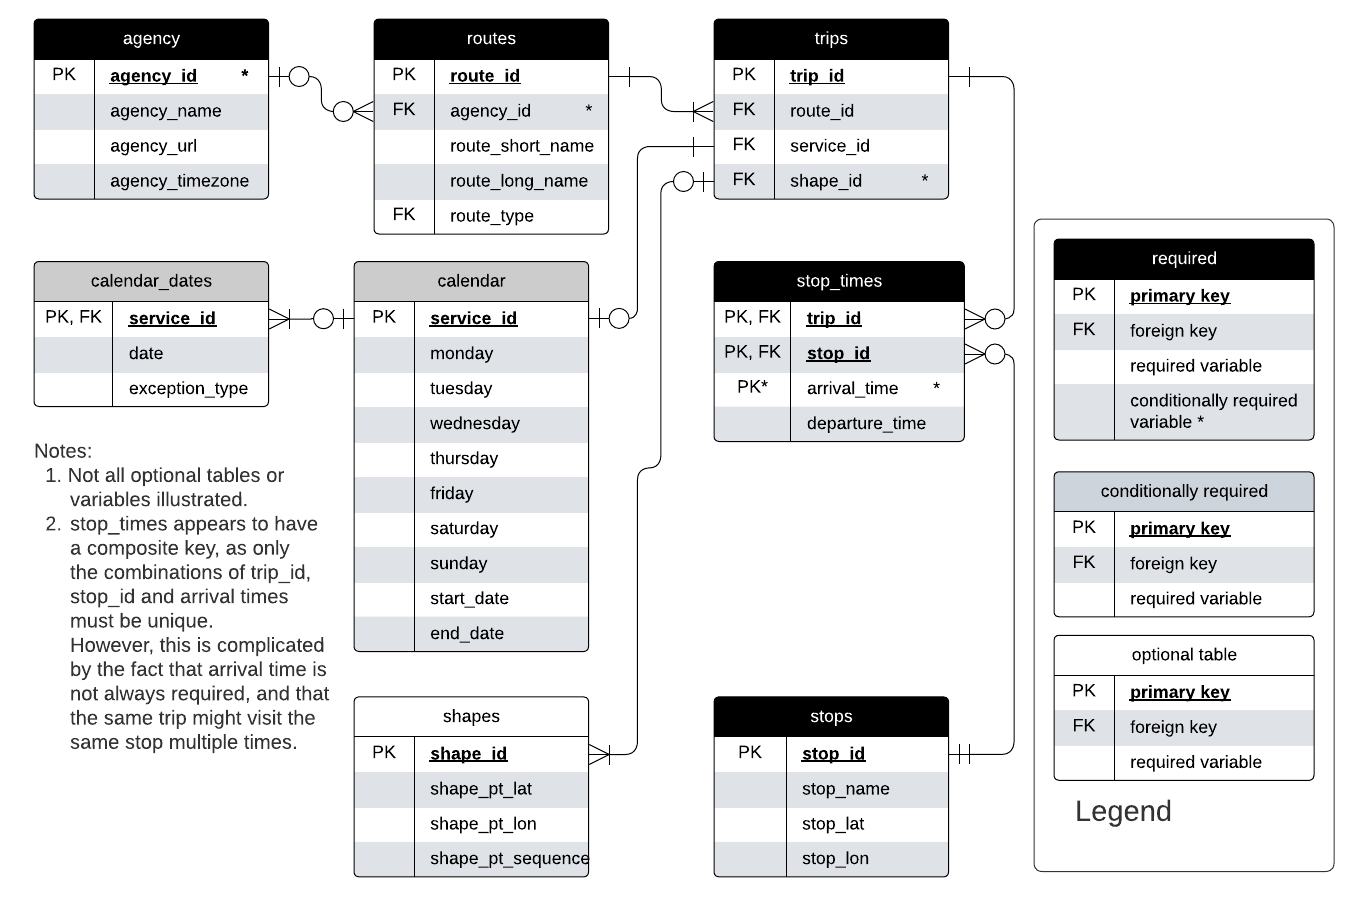
\includegraphics[width=1\linewidth]{graphics/GTFS} \caption{GTFS entity relationship diagram. Source: adapted by author from Alamri et al (2023) and the GTFS Schedule Reference (16/11/2023 revision).}\label{fig:GTFS_ERD}
\end{figure}

GTFS allows individual transit systems to be included in many online
products and analysis, including the Transit Score metric itself.
\citet{Wong:2013aa} provides another example of what can be done with
GTFS data, having developed code to calculate of some of the TCQSM
metrics and compared these across 50 transit operators. The
\citet{Wong:2013aa} code is readily available (
https://github.com/jcwong86/GTFS\_Explore\_Tool),\\
but does not appear to be currently maintained. Future research may
involve reviewing this code and using it to analyse modern GTFS feeds,\\
but in this paper the aim is more modest, being to use GTFS data to
calculate Currie and Senbergs' (2007) SI.

\hypertarget{the-transit-suppy-index}{%
\subsection{The Transit Suppy Index}\label{the-transit-suppy-index}}

Currie and Senbergs' (2007) focus was the context of Melbourne's Census
Collection Districts (CCD) and calculations based on a week of transit
service. A more generalized form of the Transit Supply Index (SI) is
shown below:

\[SI_{area, time} = \sum{\frac{Area_{Bn}}{Area_{area}}*SL_{n, time}}\]

\begin{enumerate}
\def\labelenumi{(\arabic{enumi})}
\tightlist
\item
  \(SI_{area, time}\) is the Supply Index for the area of interest and a
  given period of time;
\item
  \(Area_{Bn}\) is the buffer area for each stop (n) within the area of
  interest. In Currie and Senbergs (2007) this was based on a radius of
  400 metres for bus and tram stops, and 800 metres for railway
  stations;
\item
  \(Area_{area}\) is the area of the area of interest; and
\item
  \(SL_{n,time}\) is the number of transit arrivals for each stop for a
  given time period.
\end{enumerate}

An advantage of the SI is that it is a relatively simple number to
calculate, understand and explain. It describes the number of transit
arrivals at stops within an area of interest and time frame, multiplied
by a factor accounting for the proportion of the area of interest that
is within typical walking distances of each stop. Hence, more services,
more stops and higher frequencies increase the score.

The SI score does not incorporate service span, speed or other elements
of a transit service. While these can be important to passenger
experience, they might add complexity. Simplicity is also helped by the
way that the SI is additive, in that \(SI_{area, time}\) scores can be
aggregated to calculate an overall score across multiple time periods or
for a region encompassing multiple areas of interest.

\hypertarget{methodology}{%
\section{Methodology}\label{methodology}}

This study developed a package with tools for calculating the SI from
GTFS data. The R programming language \citep{R-base}, was adopted for
code development, and the package development setup and workflow
described by \citet{wickham2023r} was adopted. Various existing packages
were relied upon including: the sf package \citep{R-sf} for geospatial
analysis; the tidyverse \citep{tidyverse2019}; gtfstools
\citep{R-gtfstools}; and tidytransit \citep{R-tidytransit}. Some code
was adapted from examples, vignettes and other documentation in the
tidytransit, gtfstools and other packages.

Two cases where used during the code development and testing such that
results might be generated for real GTFS data: the Mornington Peninsula
Tourist Railway GTFS feed and the Public Transport Victoria (PTV) GTFS
feed, both in Victoria, Australia. Both were selected primarily for
convenience, given that the authors are familiar with the typical
service patterns and geography.

Figure @ref(Melbourne\_map)) shows the areas of interest for which
results are presented in this paper, including Greater Melbourne and its
SA3 zones (main), SA1 zones in the central part of Melbourne (top-right)
and the Mornington Peninsula Railway and SA1 zones within 800 metres
(bottom-right) . Stations are shown in

\begin{figure}
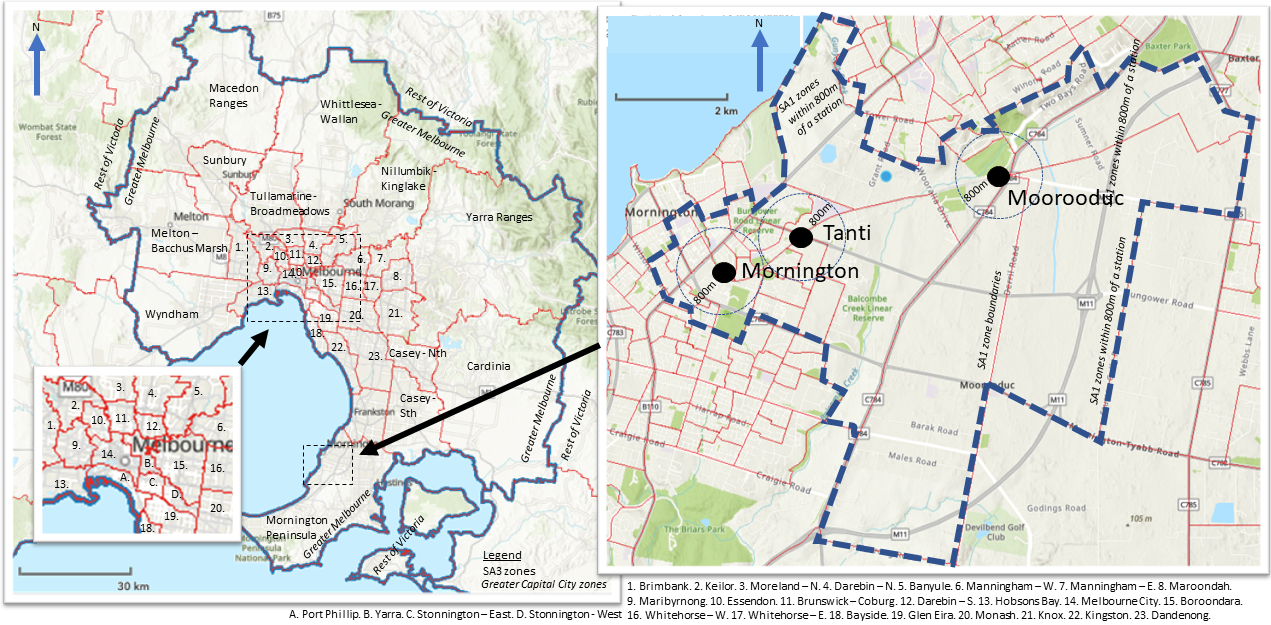
\includegraphics[width=1\linewidth]{graphics/all_maps} \caption{Areas of interest}\label{fig:Melbourne_map}
\end{figure}

Further cases were selected as leading, representative and contrasting
examples for the results reported here.

\hypertarget{mornington-penninsula-tourist-railway}{%
\subsection{Mornington Penninsula Tourist
Railway}\label{mornington-penninsula-tourist-railway}}

The Morning Peninsula Tourist Railway is in the outer south-east of
Melbourne, running on Sundays and Wednesdays between Mornington and
Moorooduc, with an intermediate stop at Tanti Park (see
https://transitfeeds.com/p/mornington-railway/806/latest/stops). A GTFS
feed from 2018 was selected for the purposes of tests and demonstrating
the code and output. Australian Bureau of Statistics (ABS) data was also
used, sources via the strayr and absmapsdata packages \citep{r-strayr}.
The Mornington Peninsular Statistical Area 3 (SA3) zone and the
Statistical Area 1 (SA1) zones contained within it were adopted as the
areas of interest. These are shown in Figure
@ref(fig:mornington\_map\_ABS), together with the locations of the three
railway stations.

\hypertarget{public-transport-victoria-ptv}{%
\subsection{Public Transport Victoria
(PTV)}\label{public-transport-victoria-ptv}}

Larger scale testing was performed using the Victorian GTFS feed,
published by Public Transport Victoria (PTV), sourced via
\citet{transitfeeds_victoria:2023aa} for historical feeds. Again, ABS
data was used as the areas of interest, focusing on SA1 zones within
Greater Melbourne. Data was analysed for the second Tuesday in August
each year, so as to match the typical date of the Australian census.

\hypertarget{results}{%
\section{Results}\label{results}}

\hypertarget{code-structure}{%
\subsection{Code structure}\label{code-structure}}

\begin{figure}
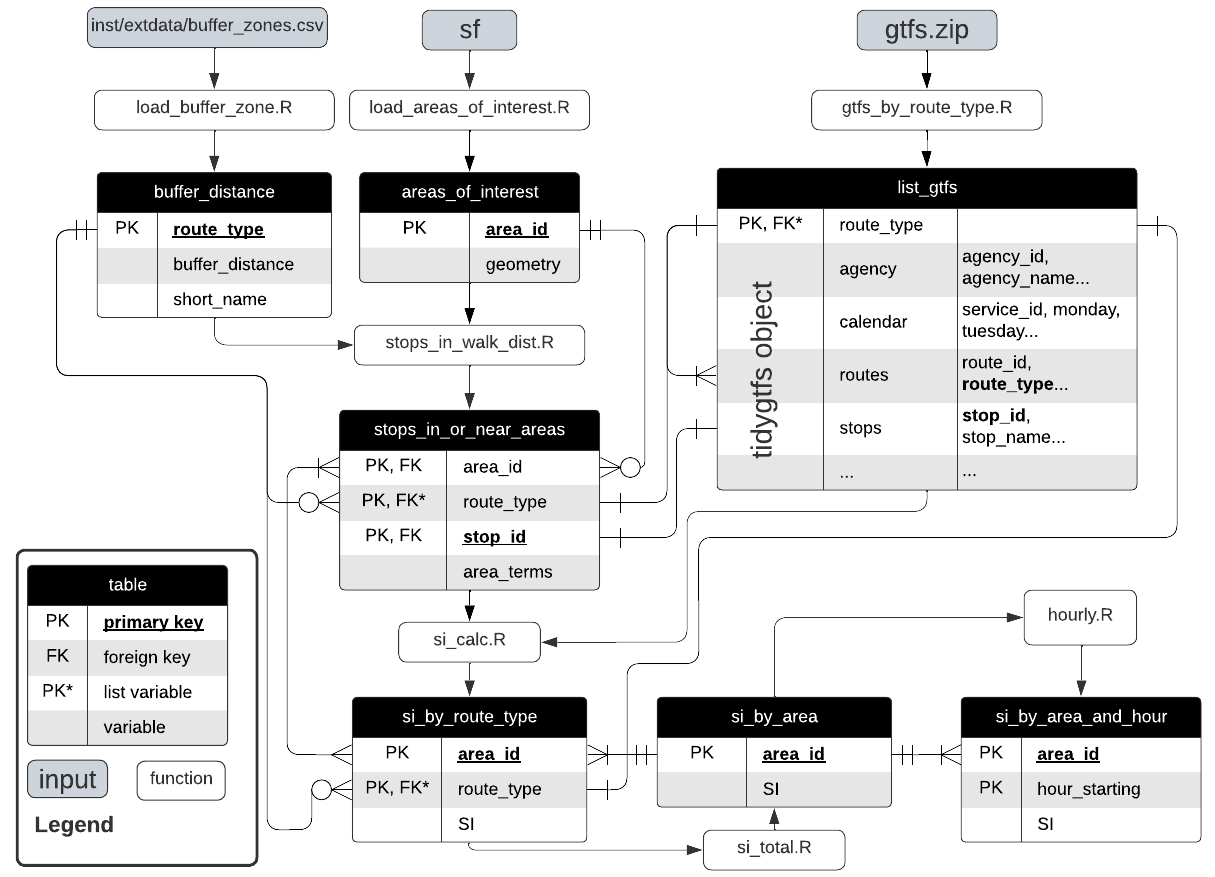
\includegraphics[width=1\linewidth]{graphics/SI_data_structure} \caption{Entity Relationship Diagram (ERD) showing the data structure and functions related to the gtfssupplyindex package}\label{fig:SI_ERD}
\end{figure}

Developed code is available and documented on github
\citep{gtfssupplyindex_github}. The structure of the package, functions
developed, and data tables are shown in Figure @ref(fig:SI\_ERD), which
shows\\
how the package takes input from three files: a gtfs feed (gtfs.zip); a
sf object describing the geometry of the areas for which the SI is to be
calculated; and a csv file defining the buffer zone distances (in
metres) for each route type\footnote{This file is included in the
  package.}. The ultimate output is a si\_by\_area\_and\_hour table,
which reports the SI score for each hour of the day across dates
specified by the user.

\hypertarget{mornington-pennisula-tourist-railway}{%
\subsection{Mornington Pennisula Tourist
Railway}\label{mornington-pennisula-tourist-railway}}

The various functions and their output and explained in the following,
using the Mornington Peninsula GTFS for December 30th, 2018, and SA1
zone boundaries. Individual steps are:

\begin{enumerate}
\def\labelenumi{(\arabic{enumi})}
\item
  loading the gtfs.zip file: the gtfs\_by\_route\_type function loads
  the gtfs data and splits it into a list (by route\_type) of tidygtfs
  objects, using the filter\_by\_route\_type function from the gtfstools
  package \citep{filter_GTFS_by_mode}.
\item
  loading geometry information about the areas of interest: geographical
  data about the areas of interest are loaded by the
  load\_areas\_of\_interest.R function into an sf object, using the sf
  package \citep{R-sf}. The resultant areas\_of\_interest table contains
  each area\_id and its associated geometry. Data about buffer zones,
  specifically the walking distance threshold assigned to each
  route\_type (mode) is then loaded, again through a function
  (load\_buffer\_zone.R).
\item
  calculating which stops are within the catchment walking distance of
  which areas: using the stops\_in\_walk\_dist function. Figure
  @ref(fig:calculate\_stop\_in\_or\_near\_areas\_verbose)) shows an
  intermediate step in this is function, in which the SA1 areas within
  the 800 metre catchment of the Mornington stations is identifed.
\end{enumerate}

\begin{figure}
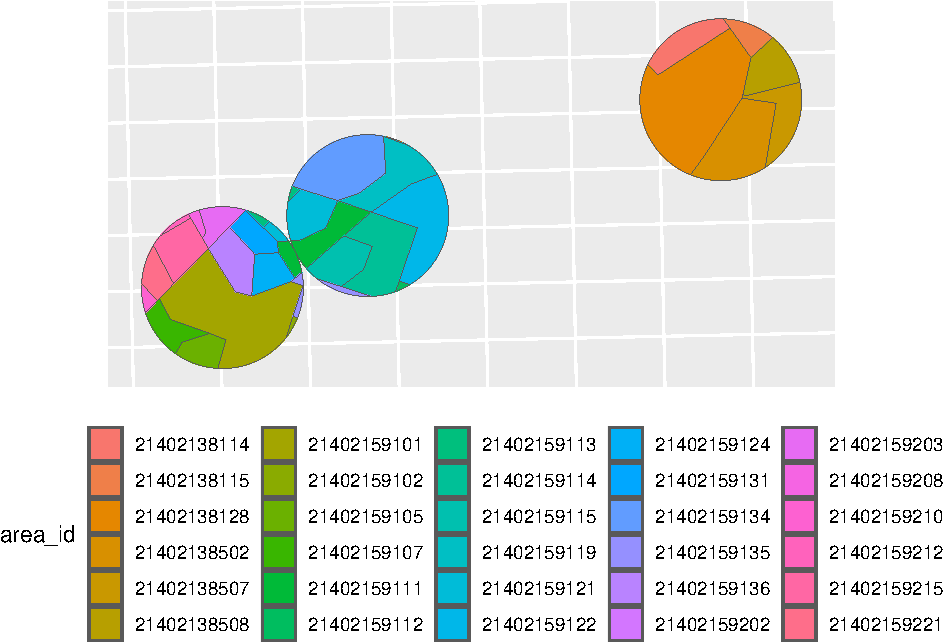
\includegraphics[width=1\linewidth]{Leveraging_GTFS_to_assess_transit_supply_Transport_Geography_files/figure-latex/calculate_stop_in_or_near_areas_verbose-1} \caption{Step 3, stop catchments for the Mornington Penninsula Tourist Railway, showing intersections with SA1 zones}\label{fig:calculate_stop_in_or_near_areas_verbose}
\end{figure}

\begin{enumerate}
\def\labelenumi{(\arabic{enumi})}
\setcounter{enumi}{3}
\tightlist
\item
  Calculating SI scores for a given time period: using the si\_calc.R
  function. This adapts code from an article included in the tidytransit
  package \citep{tidytransit_departure_timetable} to calculate the
  number of arrivals in a given time period, and combines this with the
  calculated area components. The si\_total.R and hourly.R functions
  provided aggregation, giving the results shown in Table
  @ref(tab:SI\_mornington\_20181230\_output) and mapped in Figure
  @ref(fig:SI\_mornington\_20181230\_output).
\end{enumerate}

\begin{figure}
\centering
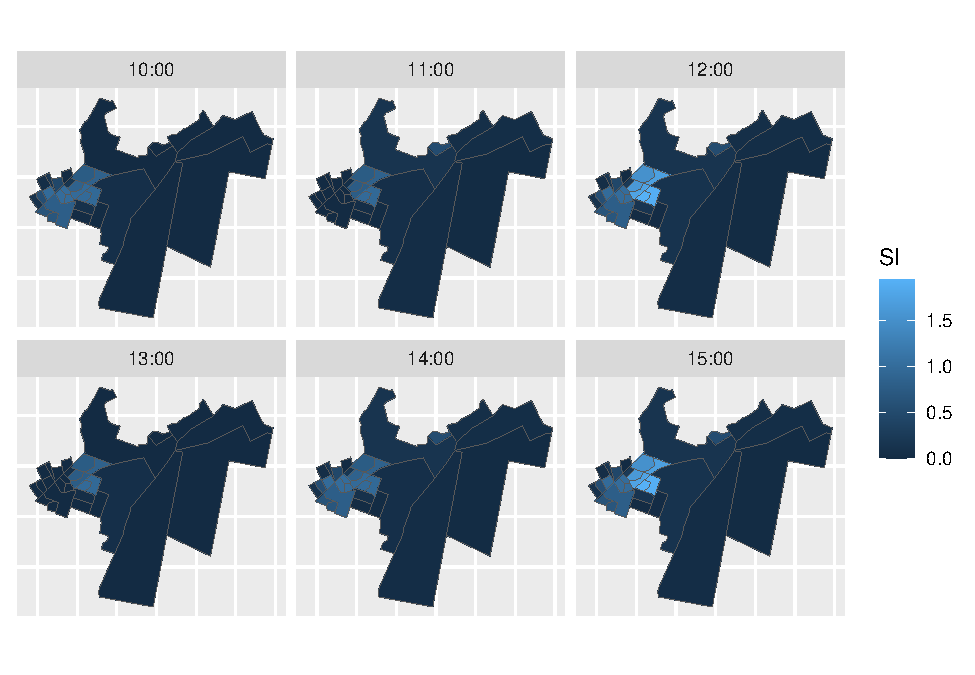
\includegraphics{Leveraging_GTFS_to_assess_transit_supply_Transport_Geography_files/figure-latex/SI_mornington_20181230_output-1.pdf}
\caption{Mornington Penninsula Tourist Railway hourly SI values for
December 30, 2018}
\end{figure}

\hypertarget{central-melbourne}{%
\subsection{Central Melbourne}\label{central-melbourne}}

Figure @ref(Melbourne\_CBD\_map\_230808) shows SI scores for Tuesday
August 8, 2023, by hour between 5am and 11am (top) and by mode for the
whole day (bottom). These generally expectations, with higher SI scores
shown in the Central Business District (CBD), where there are the five
stations that make up the City Loop: Flinders Street Station, Southern
Cross Station, Flagstaff Station, Melbourne Central Station and
Parliament Station; and where many tram and bus routes converge. The SI
scores are highest between 7-9am, reflecting the typical service peaks.
Results are also consistent with: the high number for bus services along
the Victoria and Queen Street corridors; and tram services that mostly
run along the Swanston, Elizabeth, Bourke and Collins Street corridors.

\begin{figure}
\centering
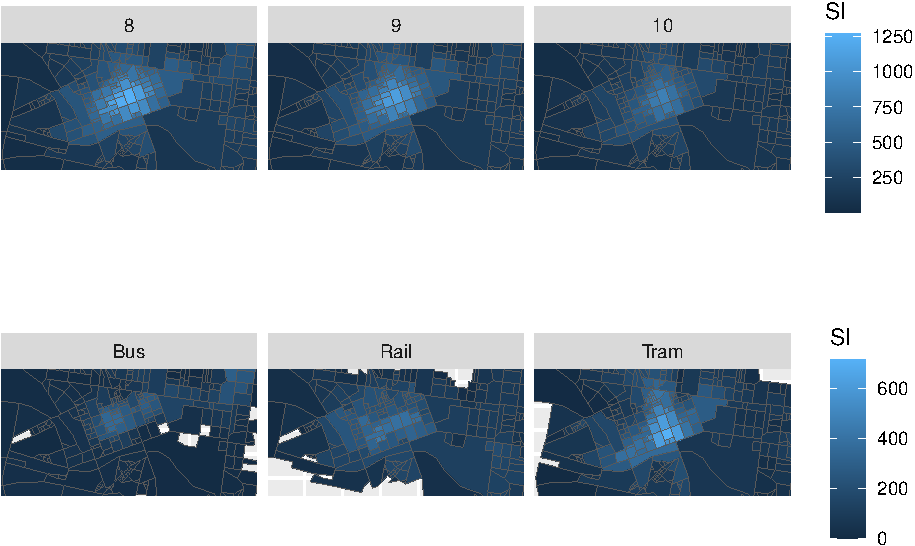
\includegraphics{Leveraging_GTFS_to_assess_transit_supply_Transport_Geography_files/figure-latex/Melbourne_CBD_map_230808-1.pdf}
\caption{Victorian GTFS and central Melbourne SA1 zones, SI values for
October 10, 2023, by hour between 5am and 11am (top) and by mode
(bottom)}
\end{figure}

\hypertarget{greater-melbourne}{%
\subsection{Greater Melbourne}\label{greater-melbourne}}

\hypertarget{by-hour}{%
\subsubsection{By hour}\label{by-hour}}

\begin{figure}
\centering
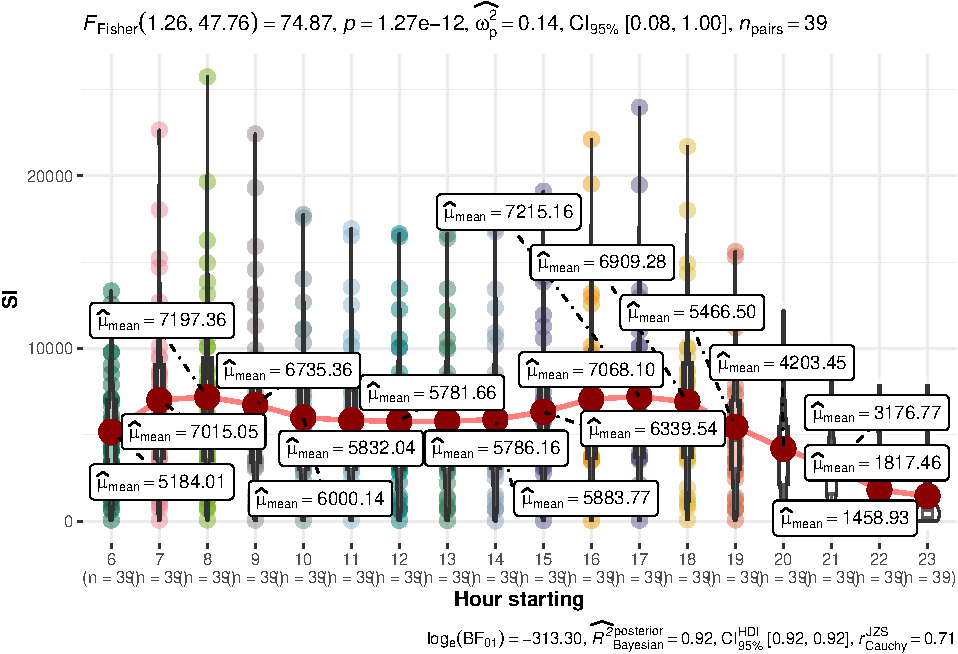
\includegraphics{Leveraging_GTFS_to_assess_transit_supply_Transport_Geography_files/figure-latex/Melbourne_230808_by_hour-1.pdf}
\caption{Victorian GTFS and SA3 zones, SI values for Tuesday August 8,
2023, by hour, 5am to midnight}
\end{figure}

\hypertarget{location-population-and-equality-of-service}{%
\subsubsection{Location, population and equality of
service}\label{location-population-and-equality-of-service}}

\begin{figure}
\centering
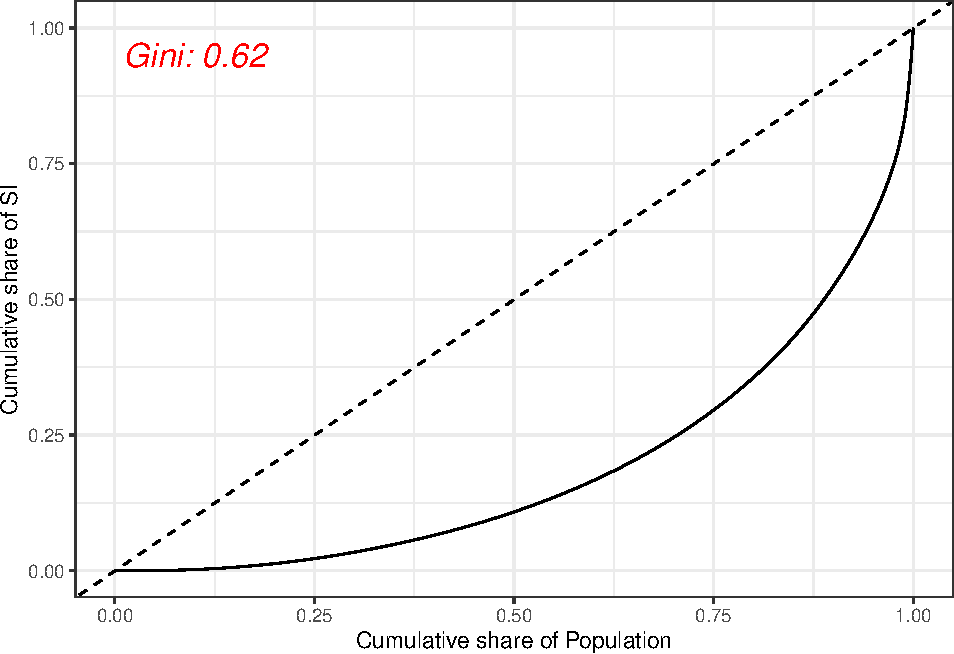
\includegraphics{Leveraging_GTFS_to_assess_transit_supply_Transport_Geography_files/figure-latex/Gini_coefficients-1.pdf}
\caption{Victorian GTFS and SA1 zones within Greater Melbourne, SI
values for Tuesday August 8, 2023, Lorenz plot}
\end{figure}

\begin{tabular}{l|c}
\hline
**Characteristic** & **N = 40**\\
\hline
Population & \\
\hline
Median (IQR) & 104,332 (77,574, 156,285)\\
\hline
Skew & 1\\
\hline
Mean (SD) & 118,389 (59,360)\\
\hline
10\%, 90\% & 52,168, 193,124\\
\hline
5\%, 95\% & 41,080, 218,426\\
\hline
1\%, 99\% & 25,502, 264,363\\
\hline
Range & 25,146, 279,213\\
\hline
SI & \\
\hline
Median (IQR) & 94,230 (53,209, 136,011)\\
\hline
Skew & 5\\
\hline
Mean (SD) & 132,633 (208,439)\\
\hline
10\%, 90\% & 17,527, 220,764\\
\hline
5\%, 95\% & 12,483, 289,046\\
\hline
1\%, 99\% & 5,282, 938,342\\
\hline
Range & 839, 1,335,114\\
\hline
\end{tabular}

\begin{figure}
\centering
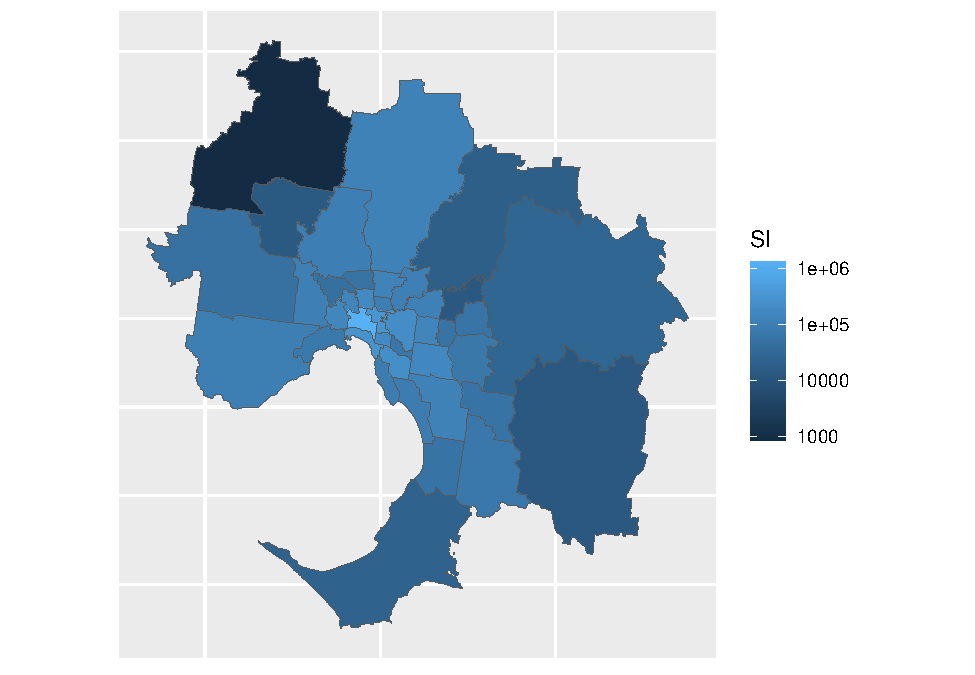
\includegraphics{Leveraging_GTFS_to_assess_transit_supply_Transport_Geography_files/figure-latex/map_greater_melbourne_230808_by_sa3-1.pdf}
\caption{Victorian GTFS and SA3 zones within Greater Melbourne, SI
values for Tuesday August 8, 2023 (top), 2021 census population
(middle), and SI divided by population (bottom)}
\end{figure}

\begin{figure}
\centering
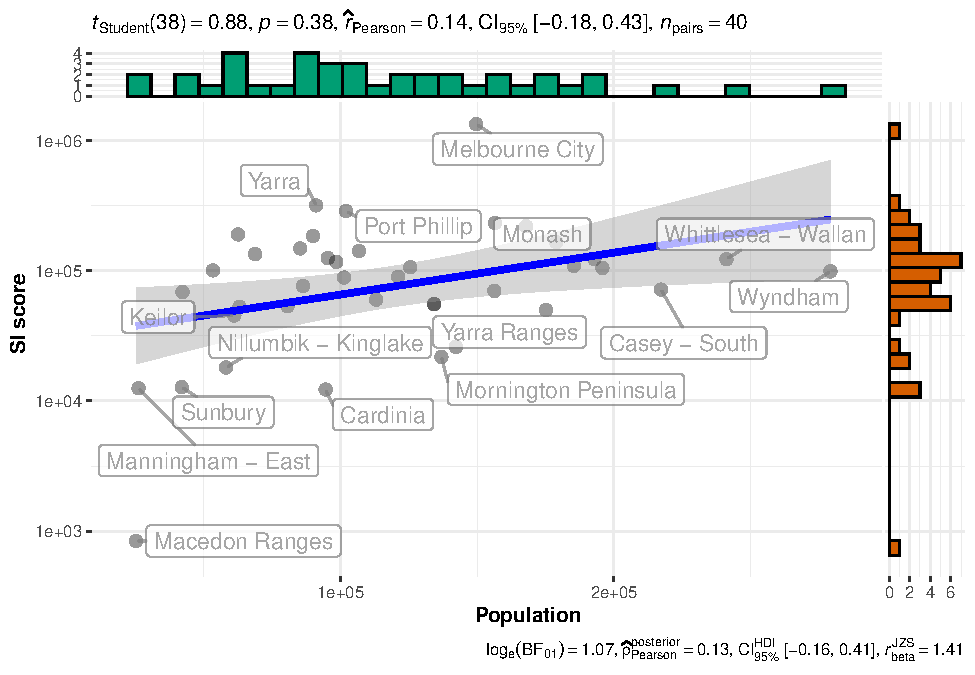
\includegraphics{Leveraging_GTFS_to_assess_transit_supply_Transport_Geography_files/figure-latex/greater_melbourne_230808_by_sa3_scatterplot-1.pdf}
\caption{Victorian GTFS and SA3 zones within Greater Melbourne, SI
values for Tuesday August 8, 2023 (top), 2021 census population
(middle), and SI divided by population (bottom)}
\end{figure}

\hypertarget{trends}{%
\subsection{Trends}\label{trends}}

\hypertarget{extensions}{%
\section{Extensions}\label{extensions}}

\hypertarget{melbourne-cbd-index}{%
\subsection{Melbourne CBD Index}\label{melbourne-cbd-index}}

\hypertarget{new-york-index}{%
\subsection{New York Index}\label{new-york-index}}

\hypertarget{london-index}{%
\subsection{London Index}\label{london-index}}

\hypertarget{discussion-and-conclusions}{%
\section{Discussion and conclusions}\label{discussion-and-conclusions}}

\renewcommand\refname{References}
\bibliography{References.bib, packages.bib}


\end{document}
